\chapter{系统工作流程与实证分析}
\section{系统整合}
基于前几章的描述,我们可以综合构建一个数据挖掘系统,发现用户兴趣,推荐相关内容。
整体系统流程如下图

\usetikzlibrary{shapes,snakes}
\usetikzlibrary{arrows, decorations.markings}

\tikzstyle{vecArrow} = [thick, decoration={markings,mark=at position
   1 with {\arrow[semithick]{open triangle 60}}},
   double distance=1.4pt, shorten >= 5.5pt,
   preaction = {decorate},
   postaction = {draw,line width=1.4pt, white,shorten >= 4.5pt}]

% Define box and box title style
\tikzstyle{mybox} = [draw=black, fill=white, very thick,
    rectangle, rounded corners, inner sep=10pt, inner ysep=20pt]
\tikzstyle{fancytitle} =[fill=red, text=white]

\def\html{
    \draw[rounded corners=0.1ex,fill=white,thick] (0.2,0.2) rectangle (1.2,1.5);
    \draw[rounded corners=0.1ex,fill=white,thick] (0.1,0.1) rectangle (1.1,1.4);
    \draw[rounded corners=0.1ex,fill=white,thick] (0,0) rectangle (1,1.3);
    \node at (0.5,0.3) {\tiny HTML};
}


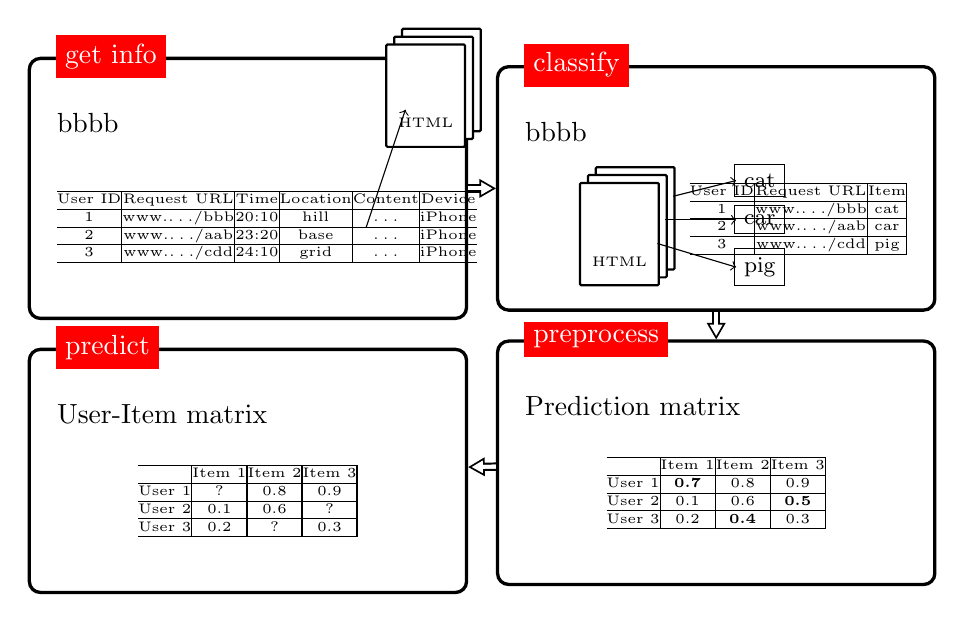
\begin{tikzpicture}
\node [mybox] (stepone){
	\begin{minipage}{0.40\textwidth}
		bbbb
		\newline
		\tiny
        \begin{center}
		\begin{tabular}{@{} c @{}|@{} c @{}|@{} c @{}|@{} c @{}|@{} c @{}|@{} c @{}}
			\hline
			User ID & Request URL & Time & Location & Content & Device \\
			\hline
			1 & www.$\ldots$/bbb & 20:10 & hill & $\ldots$ & iPhone \\
			\hline
			2 & www.$\ldots$/aab & 23:20 & base & $\ldots$ & iPhone \\
			\hline
			3 & www.$\ldots$/cdd & 24:10 & grid & $\ldots$ & iPhone \\
			\hline
		\end{tabular}
		\end{center}
	\end{minipage}
};
\begin{scope}[xshift=50,yshift=15]
\html
\end{scope}
\draw [->] (1.5,-0.5) -- (2,1);
\node[fancytitle, right=10pt] at (stepone.north west) {get info};

\node[mybox, right=10pt] at (stepone.east) (steptwo){
	\begin{minipage}{0.40\textwidth}
		bbbb
		\newline
		\tiny
        \begin{flushright}
		\begin{tabular}{@{} c @{}|@{} c @{}|@{} c @{}|@{} c @{}|@{} c @{}|@{} c @{}}
			\hline
			User ID & Request URL & Item \\
			\hline
			1 & www.$\ldots$/bbb & cat \\
			\hline
			2 & www.$\ldots$/aab & car \\
			\hline
			3 & www.$\ldots$/cdd & pig \\
			\hline
		\end{tabular}
		\end{flushright}
	\end{minipage}
};
\begin{scope}[xshift=120,yshift=-35]
\html
\end{scope}
\node[fancytitle, right=10pt] at (steptwo.north west) {classify};

\draw [->] (5.4,-0.1) -- (6.2,0.1);
\draw [->] (5.3,-0.4) -- (6.2,-0.4);
\draw [->] (5.2,-0.7) -- (6.2,-1);
\node [draw] at (6.5,0.1) {\footnotesize cat};
\node [draw] at (6.5,-0.4) {\footnotesize car};
\node [draw] at (6.5,-1) {\footnotesize pig};

\node[mybox, below=10pt] at (stepone.south) (stepfour){
	\begin{minipage}{0.40\textwidth}
		User-Item matrix
		\newline
		\tiny
        \begin{center}
		\begin{tabular}{@{} c @{}|@{} c @{}|@{} c @{}|@{} c @{}|@{} c @{}|@{} c @{}}
			\hline
			 & Item 1 & Item 2 & Item 3 \\
			\hline
			User 1 & ? & 0.8 & 0.9 \\
			\hline
			User 2 & 0.1 & 0.6 & ? \\
			\hline
			User 3 & 0.2 & ? & 0.3 \\
			\hline
		\end{tabular}
		\end{center}
	\end{minipage}
};

\node[mybox, below=10pt] at (steptwo.south) (stepthree){
	\begin{minipage}{0.40\textwidth}
		Prediction matrix
		\newline
		\tiny
        \begin{center}
		\begin{tabular}{@{} c @{}|@{} c @{}|@{} c @{}|@{} c @{}|@{} c @{}|@{} c @{}}
			\hline
			 & Item 1 & Item 2 & Item 3 \\
			\hline
			User 1 & \textbf{0.7} & 0.8 & 0.9 \\
			\hline
			User 2 & 0.1 & 0.6 & \textbf{0.5} \\
			\hline
			User 3 & 0.2 & \textbf{0.4} & 0.3 \\
			\hline
		\end{tabular}
		\end{center}
	\end{minipage}
};
\node[fancytitle, right=10pt] at (stepfour.north west) {predict};
\node[fancytitle, right=10pt] at (stepthree.north west) {preprocess};

\draw[vecArrow] (stepone) to (steptwo);
\draw[vecArrow] (steptwo) to (stepthree);
\draw[vecArrow] (stepthree) to (stepfour);
\end{tikzpicture}

窗口化时序数据训练,或者按照新闻衰减度给旧数据安排小的权值

\section{真实数据测试}
抱歉暂时没申请到机器以及数据